\documentclass[border=8pt]{standalone}
\usepackage{amsmath,amssymb}
\usepackage{tikz}
\begin{document}
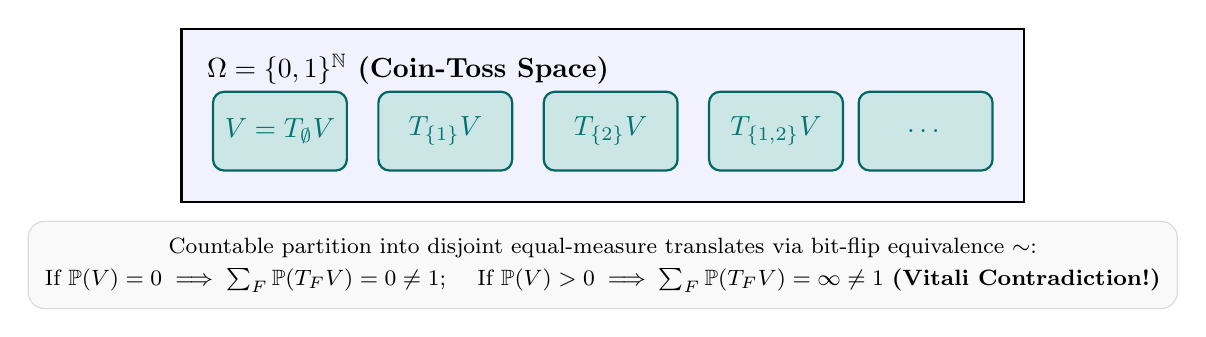
\begin{tikzpicture}[font=\small]
  \draw[thick, fill=blue!5] (0, 0) rectangle (10.7, 2.2);
  \node[anchor=north west, font=\bfseries] at (0.2, 2.0) {$\Omega = \{0,1\}^{\mathbb{N}}$ (Coin-Toss Space)};

  \foreach \x/\label in {0.4/$V = T_\emptyset V$, 2.5/$T_{\{1\}} V$, 4.6/$T_{\{2\}} V$, 6.7/$T_{\{1,2\}} V$, 8.6/$\dots$} {
    \draw[thick, fill=teal!20, draw=teal!80!black, rounded corners=4pt] (\x, 0.4) rectangle (\x+1.7, 1.4);
    \node[font=\bfseries, text=teal!90!black] at (\x+0.85, 0.9) {\label};
  }

  \node[font=\footnotesize, fill=gray!5, draw=gray!30, rounded corners=6pt, inner sep=6pt, align=center] at (5.35, -0.8) 
    {Countable partition into disjoint equal-measure translates via bit-flip equivalence $\sim$:\\[2pt]
     If $\mathbb{P}(V) = 0 \implies \sum_{F} \mathbb{P}(T_F V) = 0 \ne 1$; \quad If $\mathbb{P}(V) > 0 \implies \sum_{F} \mathbb{P}(T_F V) = \infty \ne 1$ \textbf{(Vitali Contradiction!)} };
\end{tikzpicture}
\end{document}
